\newthought{Loop invariants} and a constraint relaxation are used to solve this problem.

\vspace{10 mm}
\begin{problem}
Show that an integer is divisible by three iff the sum of its digits in decimal representation is divisible by three.
\end{problem}

The following proof is a delightful example of unconventional thinking\footnote{Unfortunately I don't know the origin of this proof and I don't remember where I first saw it.}.

We have to work with the digits in decimal representation of some integer $n$. Let's denote with $s(n)$  the sum of those digits. We will prove something stronger than the problem:

$$
s(n) = n - 9 k, \text{ for some } k \in \mathbb{Z}
$$

The delightful twist that we are going to use is a relaxation of decimal representation: we will allow digits bigger than nine. We will then heal the representation back to decimal digits less than ten in a loop while maintaining $s(n) = n - 9 k$ as a loop invariant. 

We start with a representation with just one digit, namely $n$ itself:

$$
n = \sum_{i = 0} d_i 10^i, \text{ with } d_0 = n \text{ and } \forall i > 0: d_i = 0
$$

This is not yet a valid decimal representation if $d_0 > 9$, but the loop invariant does hold: $s(n) = \sum_{i = 0} d_i = n = n - 9 \cdot 0$. In a loop we now keep subtracting ten from $d_0$ and adding a carry-over one to $d_1$ until $d_0 \leq 9$. Each time through the loop $d_1$ increases by one and $d_0$ decreases by ten, so $s(n) = \sum_{i = 0} d_i$ decreases by nine:

\begin{align*}
d_1  & \leftarrow d_1 + 1 \\
d_0  & \leftarrow d_0 - 10 \\
s(n) & \leftarrow s(n) - 9
\end{align*}

This means the loop invariant $s(n) = n - 9 k$ is maintained during the healing of $d_0$. Eventually $d_0 \leq 9$. We then look at $d_1$ and heal it similarly, carrying over to $d_2$ and subtracting ten from it. Again the loop invariant holds. We repeat this for all digits until all are healed. The healing has to finish because $n$ is a finite integer with a finite decimal representation. In the end we have a valid decimal representation and the loop invariant still holds which proves our problem.

\begin{figure}
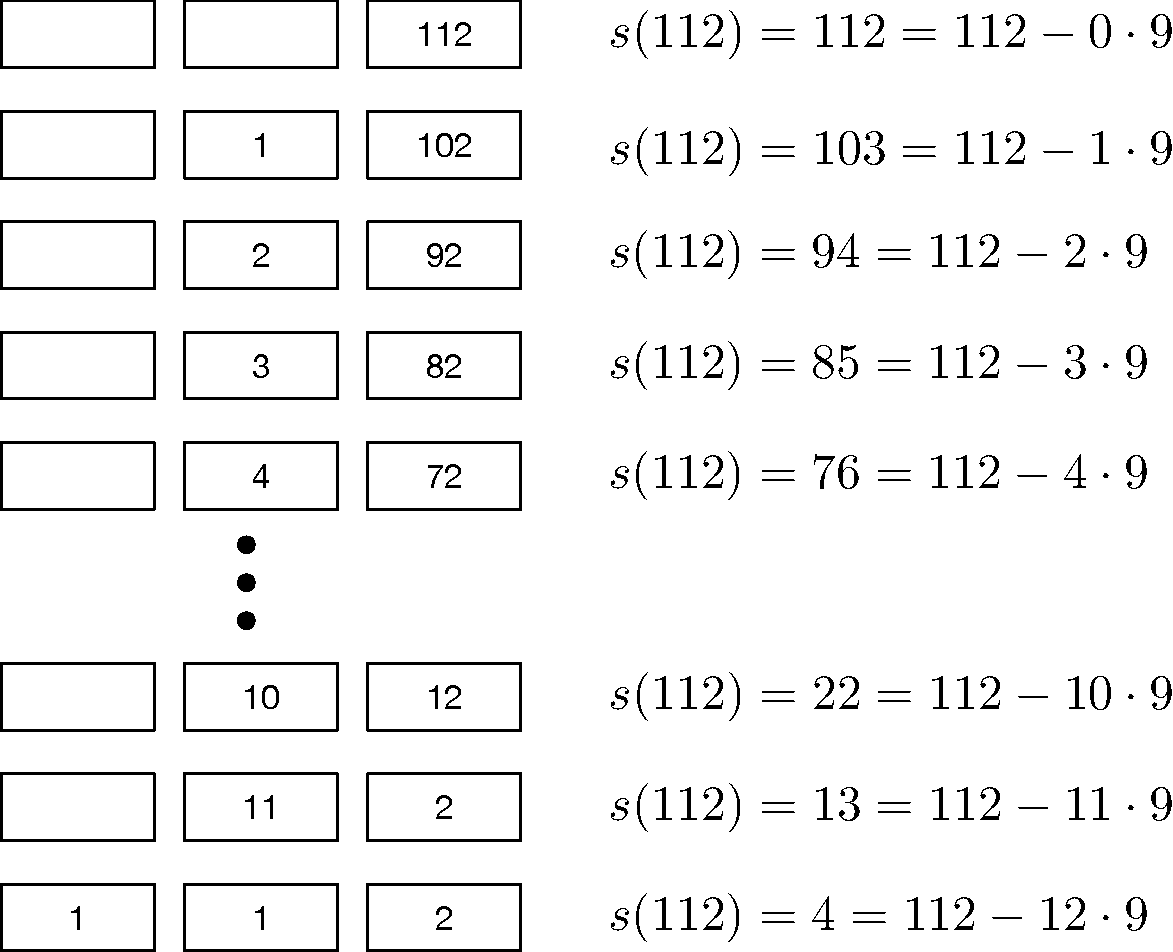
\includegraphics[scale=0.5]{example.pdf}
\caption{Example with $n=112$. In each row the boxes represent the digits in the decimal representation (least significant on the right). In the first row the representation has only one digit, the number itself. Going down, each row is one step in the healing of the representation while maintaining the loop invariant $s(112) = 112 - k \cdot 9$.}
\end{figure}

Obviously one could just observe that $10 \equiv 1 \mod 3$, so also $10^k \equiv 1 \mod 3$ and the divisibility rule follows immediately. 

$$
n = \sum_{i = 0} d_i 10^i \equiv \sum_{i = 0} d_i \mod 3
$$
